\documentclass[11pt]{article}
\usepackage[textwidth=18.0cm, textheight=23.0cm, top=2.0cm]{geometry}
\usepackage{pst-all}
\usepackage{amssymb}
\usepackage{tikz}
\usepackage{underscore}\begin{document}
\pagestyle{empty}


ClassName: \underline{\textbf{Class_10.2bp-41}}
\par
BinSize: \underline{\textbf{100 × 100}}
\par
ReduceSize: \underline{\textbf{100 × 100}}
\par
TypeNum: \underline{\textbf{99}}
\par
Num: \underline{\textbf{100}}
\par
OutS: \underline{\textbf{160000}}
\par
InS: \underline{\textbf{146010}}
\par
Rate: \underline{\textbf{0.913}}
\par
UB: \underline{\textbf{16}}
\par
LB0: \underline{\textbf{15}}
\par
LB: \underline{\textbf{16}}
\par
LBWithCut: \underline{\textbf{16}}
\par
NodeCut: \underline{\textbf{0}}
\par
ExtendedNodeCnt: \underline{\textbf{1}}
\par
GenNodeCnt: \underline{\textbf{1}}
\par
PrimalNode: \underline{\textbf{0}}
\par
ColumnCount: \underline{\textbf{78}}
\par
TotalCutCount: \underline{\textbf{0}}
\par
RootCutCount: \underline{\textbf{0}}
\par
LPSolverCnt: \underline{\textbf{62}}
\par
PricingSolverCnt: \underline{\textbf{62}}
\par
BranchAndBoundNum: \underline{\textbf{1}}
\par
isOpt: \underline{\textbf{false}}
\par
TimeOnInitSolution: \underline{\textbf{120.020 s}}
\par
TimeOnPrimal: \underline{\textbf{0.000 s}}
\par
TimeOnPricing: \underline{\textbf{3603.875 s}}
\par
TimeOnRmp: \underline{\textbf{0.110 s}}
\par
TotalTime: \underline{\textbf{3724.082 s}}
\par
\newpage


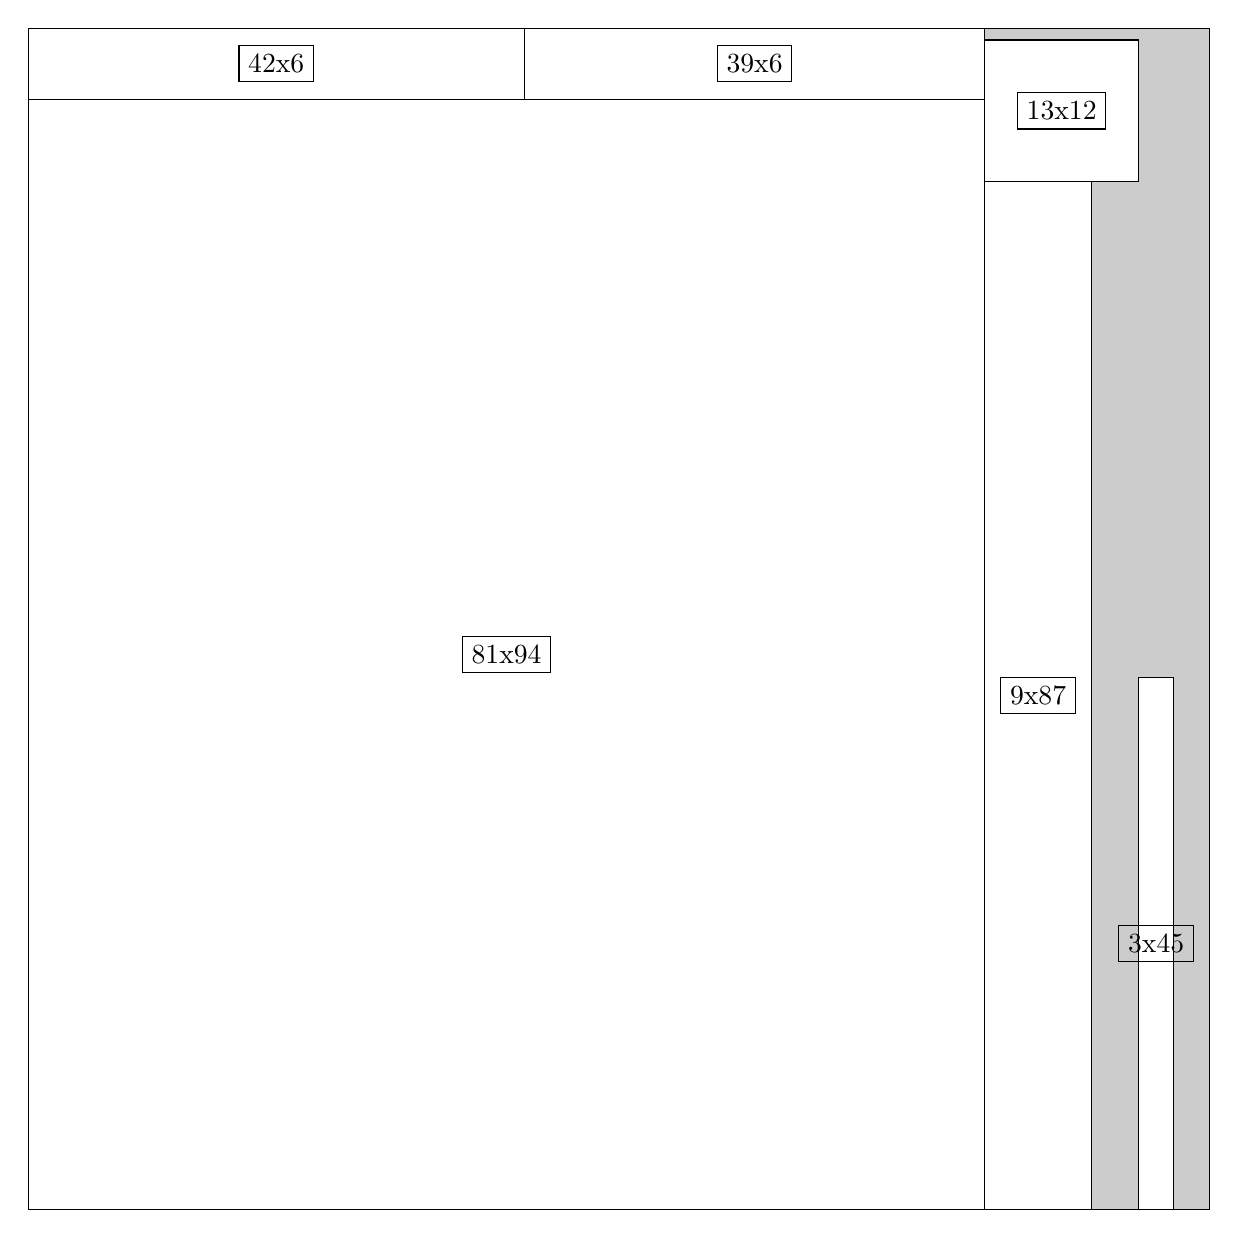
\begin{tikzpicture}[shorten >=1pt,scale=1.0,every node/.style={scale=1.0},->]
\tikzstyle{vertex}=[circle,fill=black!25,minimum size=14pt,inner sep=0pt]
\filldraw[fill=gray!40!white, draw=black] (0,0) rectangle (15.0,15.0);
\foreach \name/\x/\y/\w/\h in {81x94/0.0/0.0/12.15/14.1,9x87/12.15/0.0/1.3499999999999999/13.049999999999999,42x6/0.0/14.1/6.3/0.8999999999999999,39x6/6.3/14.1/5.85/0.8999999999999999,13x12/12.15/13.049999999999999/1.95/1.7999999999999998,3x45/14.1/0.0/0.44999999999999996/6.75}
\filldraw[fill=white!40!white, draw=black] (\x,\y) rectangle node[draw] (\name) {\name} ++(\w,\h);
\end{tikzpicture}


w =81 , h =94 , x =0 , y =0 , v =7614
\par
w =9 , h =87 , x =81 , y =0 , v =783
\par
w =42 , h =6 , x =0 , y =94 , v =252
\par
w =39 , h =6 , x =42 , y =94 , v =234
\par
w =13 , h =12 , x =81 , y =87 , v =156
\par
w =3 , h =45 , x =94 , y =0 , v =135
\par
\newpage


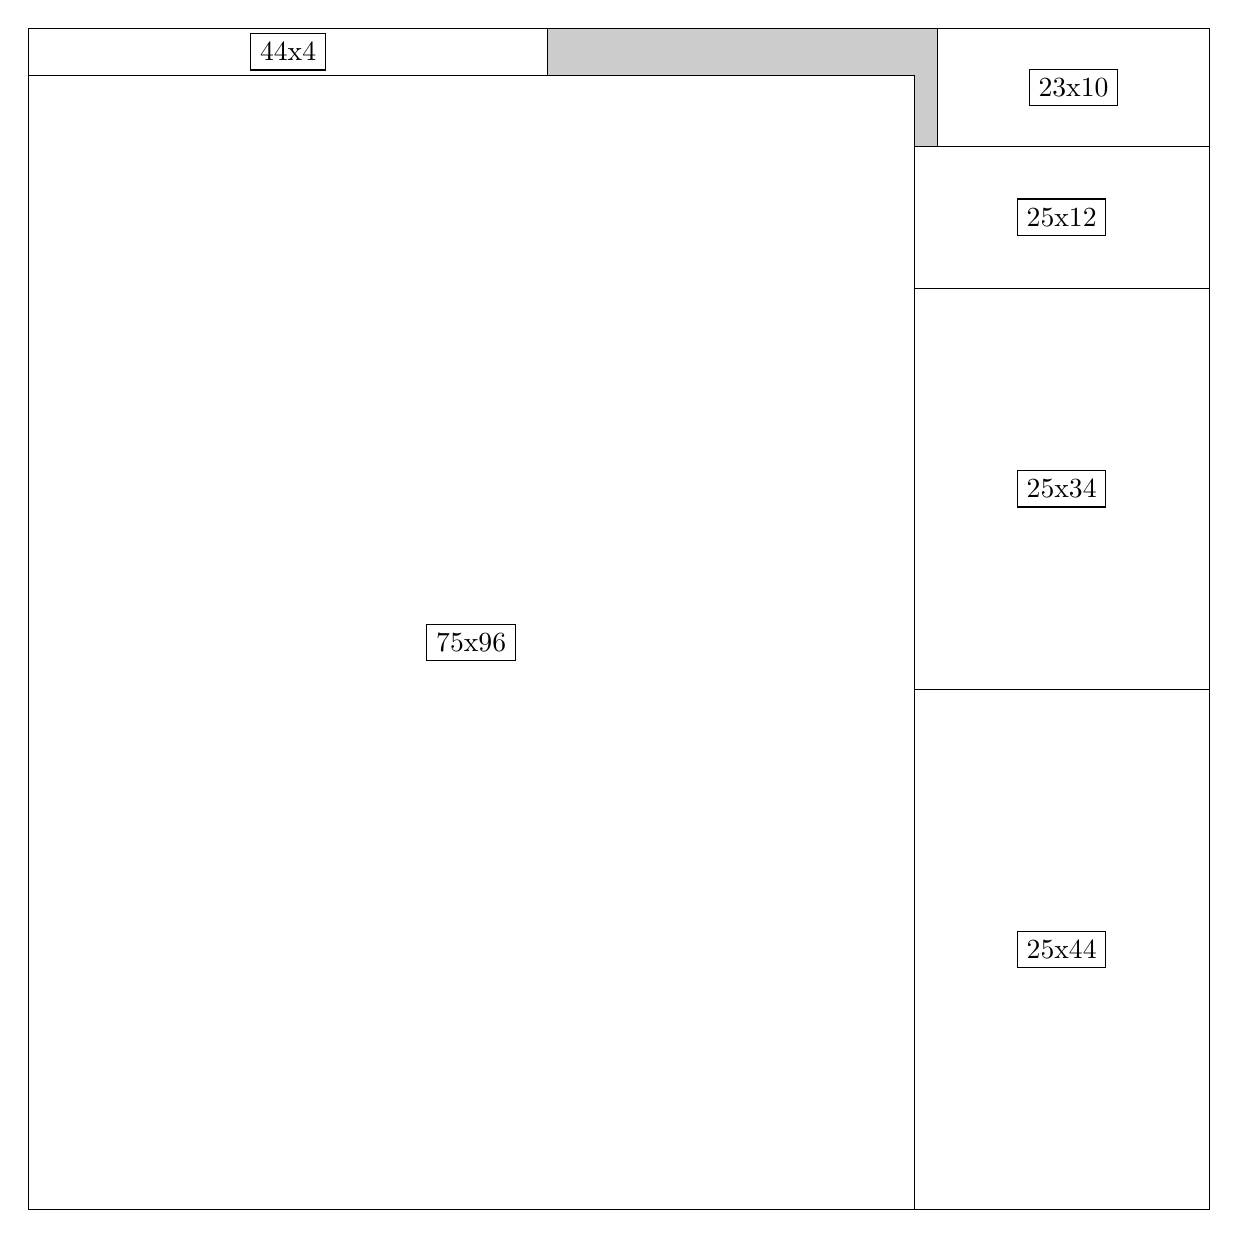
\begin{tikzpicture}[shorten >=1pt,scale=1.0,every node/.style={scale=1.0},->]
\tikzstyle{vertex}=[circle,fill=black!25,minimum size=14pt,inner sep=0pt]
\filldraw[fill=gray!40!white, draw=black] (0,0) rectangle (15.0,15.0);
\foreach \name/\x/\y/\w/\h in {75x96/0.0/0.0/11.25/14.399999999999999,25x44/11.25/0.0/3.75/6.6,25x34/11.25/6.6/3.75/5.1,25x12/11.25/11.7/3.75/1.7999999999999998,23x10/11.549999999999999/13.5/3.4499999999999997/1.5,44x4/0.0/14.399999999999999/6.6/0.6}
\filldraw[fill=white!40!white, draw=black] (\x,\y) rectangle node[draw] (\name) {\name} ++(\w,\h);
\end{tikzpicture}


w =75 , h =96 , x =0 , y =0 , v =7200
\par
w =25 , h =44 , x =75 , y =0 , v =1100
\par
w =25 , h =34 , x =75 , y =44 , v =850
\par
w =25 , h =12 , x =75 , y =78 , v =300
\par
w =23 , h =10 , x =77 , y =90 , v =230
\par
w =44 , h =4 , x =0 , y =96 , v =176
\par
\newpage


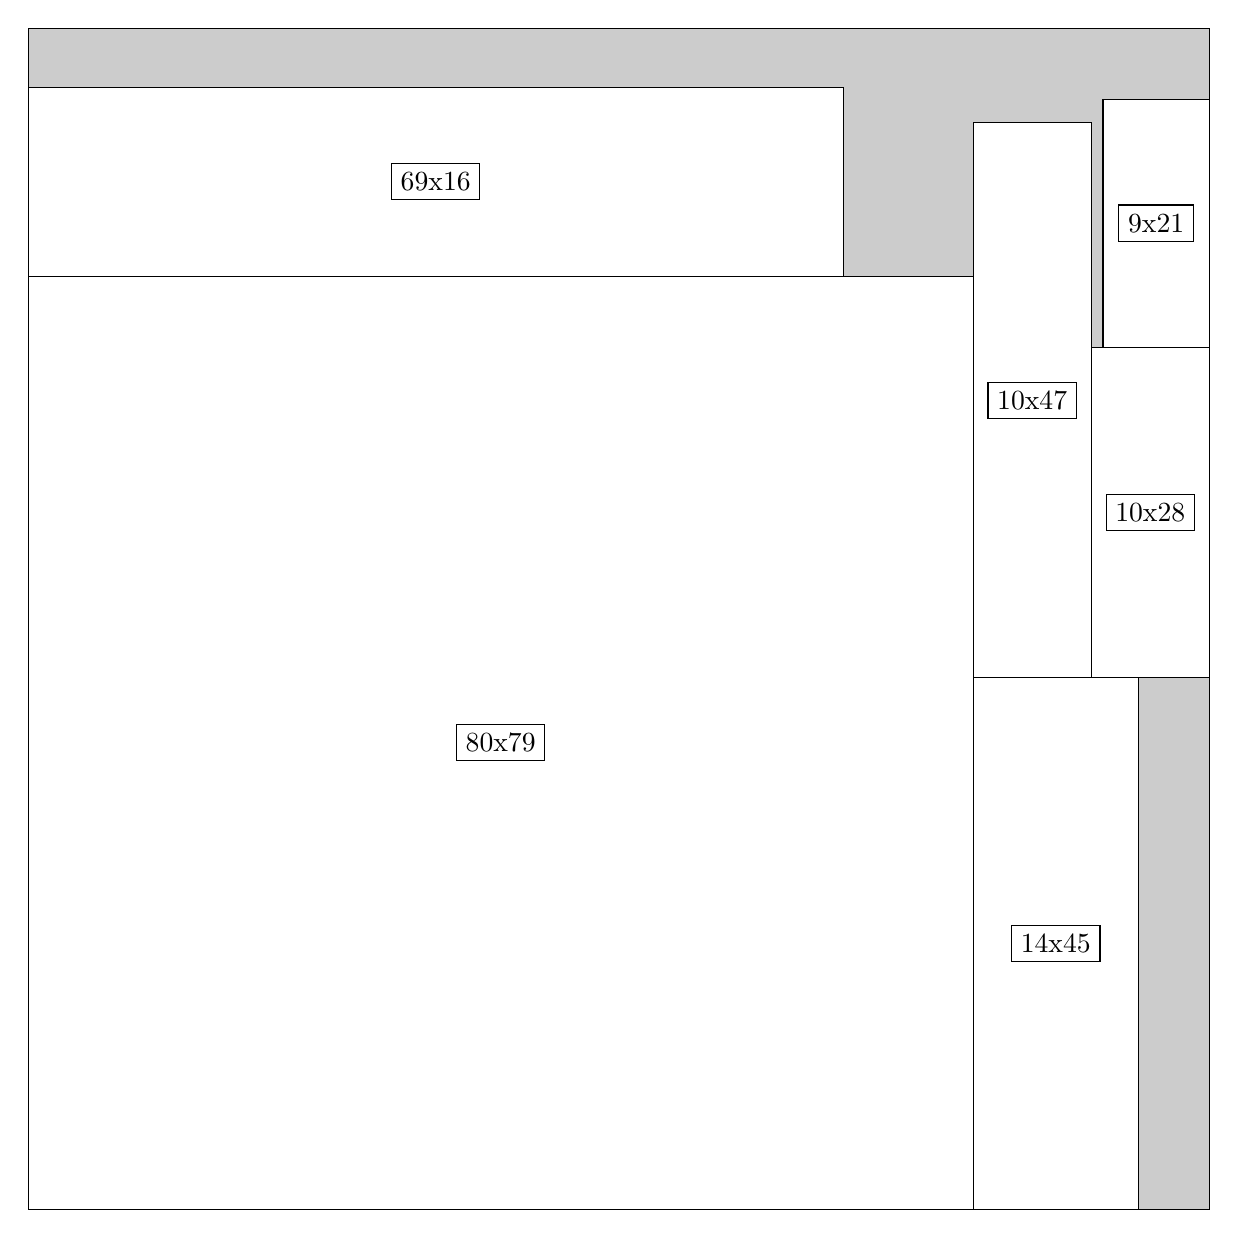
\begin{tikzpicture}[shorten >=1pt,scale=1.0,every node/.style={scale=1.0},->]
\tikzstyle{vertex}=[circle,fill=black!25,minimum size=14pt,inner sep=0pt]
\filldraw[fill=gray!40!white, draw=black] (0,0) rectangle (15.0,15.0);
\foreach \name/\x/\y/\w/\h in {80x79/0.0/0.0/12.0/11.85,69x16/0.0/11.85/10.35/2.4,14x45/12.0/0.0/2.1/6.75,10x47/12.0/6.75/1.5/7.05,10x28/13.5/6.75/1.5/4.2,9x21/13.65/10.95/1.3499999999999999/3.15}
\filldraw[fill=white!40!white, draw=black] (\x,\y) rectangle node[draw] (\name) {\name} ++(\w,\h);
\end{tikzpicture}


w =80 , h =79 , x =0 , y =0 , v =6320
\par
w =69 , h =16 , x =0 , y =79 , v =1104
\par
w =14 , h =45 , x =80 , y =0 , v =630
\par
w =10 , h =47 , x =80 , y =45 , v =470
\par
w =10 , h =28 , x =90 , y =45 , v =280
\par
w =9 , h =21 , x =91 , y =73 , v =189
\par
\newpage


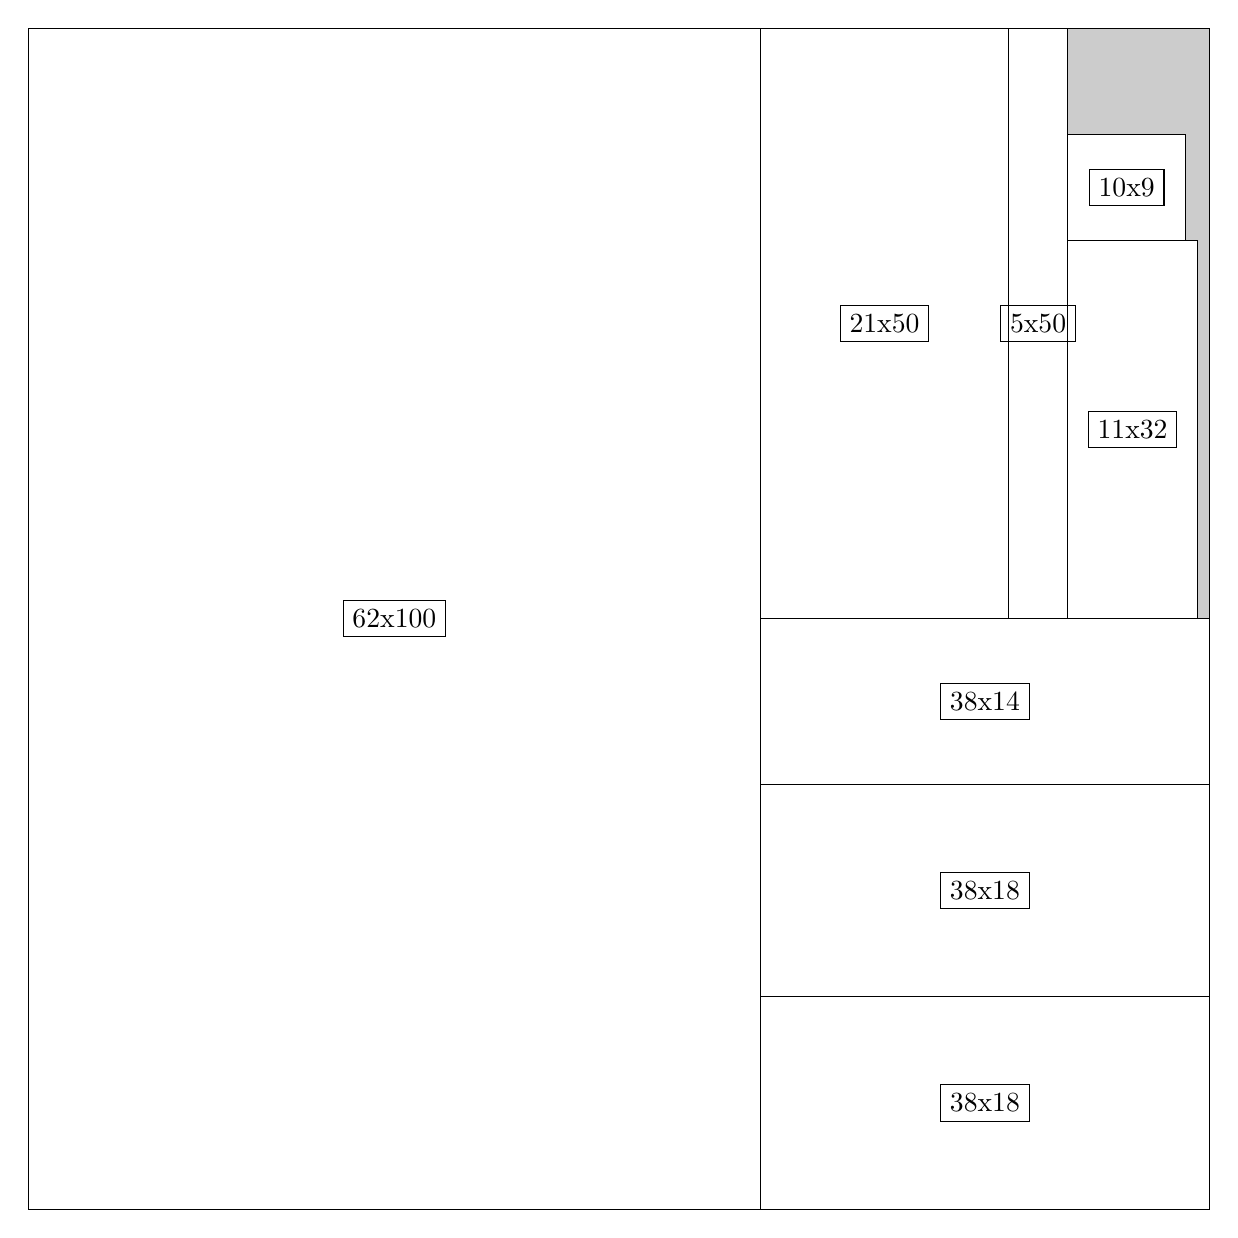
\begin{tikzpicture}[shorten >=1pt,scale=1.0,every node/.style={scale=1.0},->]
\tikzstyle{vertex}=[circle,fill=black!25,minimum size=14pt,inner sep=0pt]
\filldraw[fill=gray!40!white, draw=black] (0,0) rectangle (15.0,15.0);
\foreach \name/\x/\y/\w/\h in {62x100/0.0/0.0/9.299999999999999/15.0,21x50/9.299999999999999/7.5/3.15/7.5,38x18/9.299999999999999/0.0/5.7/2.6999999999999997,38x18/9.299999999999999/2.6999999999999997/5.7/2.6999999999999997,38x14/9.299999999999999/5.3999999999999995/5.7/2.1,11x32/13.2/7.5/1.65/4.8,5x50/12.45/7.5/0.75/7.5,10x9/13.2/12.299999999999999/1.5/1.3499999999999999}
\filldraw[fill=white!40!white, draw=black] (\x,\y) rectangle node[draw] (\name) {\name} ++(\w,\h);
\end{tikzpicture}


w =62 , h =100 , x =0 , y =0 , v =6200
\par
w =21 , h =50 , x =62 , y =50 , v =1050
\par
w =38 , h =18 , x =62 , y =0 , v =684
\par
w =38 , h =18 , x =62 , y =18 , v =684
\par
w =38 , h =14 , x =62 , y =36 , v =532
\par
w =11 , h =32 , x =88 , y =50 , v =352
\par
w =5 , h =50 , x =83 , y =50 , v =250
\par
w =10 , h =9 , x =88 , y =82 , v =90
\par
\newpage


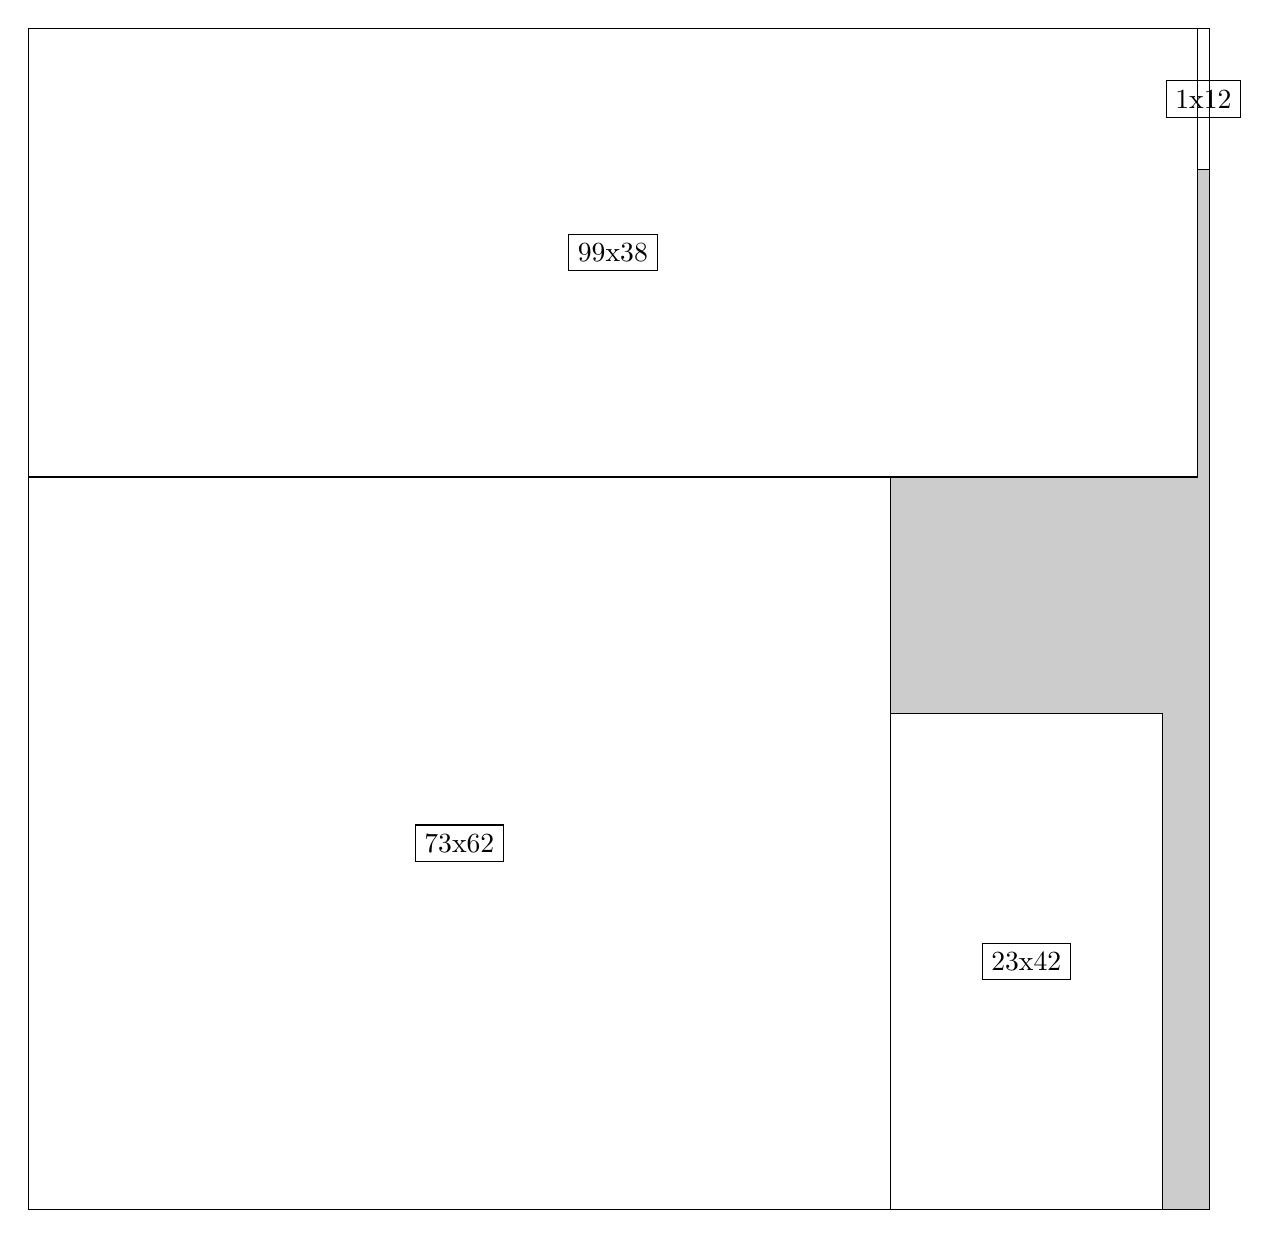
\begin{tikzpicture}[shorten >=1pt,scale=1.0,every node/.style={scale=1.0},->]
\tikzstyle{vertex}=[circle,fill=black!25,minimum size=14pt,inner sep=0pt]
\filldraw[fill=gray!40!white, draw=black] (0,0) rectangle (15.0,15.0);
\foreach \name/\x/\y/\w/\h in {73x62/0.0/0.0/10.95/9.299999999999999,99x38/0.0/9.299999999999999/14.85/5.7,23x42/10.95/0.0/3.4499999999999997/6.3,1x12/14.85/13.2/0.15/1.7999999999999998}
\filldraw[fill=white!40!white, draw=black] (\x,\y) rectangle node[draw] (\name) {\name} ++(\w,\h);
\end{tikzpicture}


w =73 , h =62 , x =0 , y =0 , v =4526
\par
w =99 , h =38 , x =0 , y =62 , v =3762
\par
w =23 , h =42 , x =73 , y =0 , v =966
\par
w =1 , h =12 , x =99 , y =88 , v =12
\par
\newpage


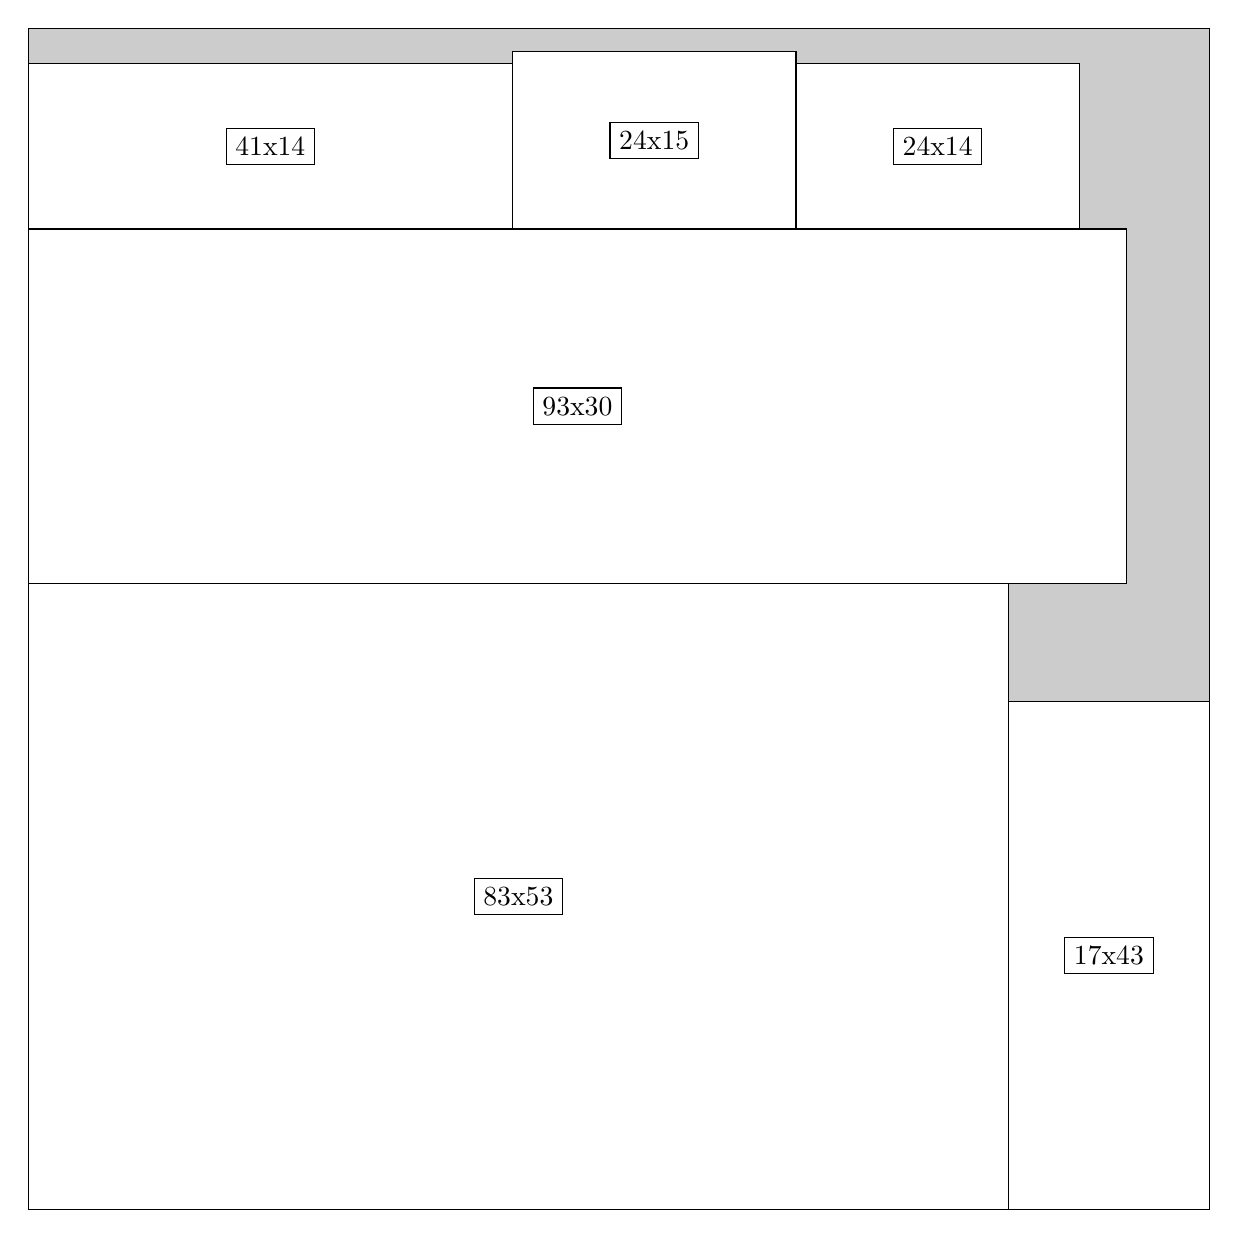
\begin{tikzpicture}[shorten >=1pt,scale=1.0,every node/.style={scale=1.0},->]
\tikzstyle{vertex}=[circle,fill=black!25,minimum size=14pt,inner sep=0pt]
\filldraw[fill=gray!40!white, draw=black] (0,0) rectangle (15.0,15.0);
\foreach \name/\x/\y/\w/\h in {83x53/0.0/0.0/12.45/7.949999999999999,93x30/0.0/7.949999999999999/13.95/4.5,17x43/12.45/0.0/2.55/6.45,41x14/0.0/12.45/6.1499999999999995/2.1,24x15/6.1499999999999995/12.45/3.5999999999999996/2.25,24x14/9.75/12.45/3.5999999999999996/2.1}
\filldraw[fill=white!40!white, draw=black] (\x,\y) rectangle node[draw] (\name) {\name} ++(\w,\h);
\end{tikzpicture}


w =83 , h =53 , x =0 , y =0 , v =4399
\par
w =93 , h =30 , x =0 , y =53 , v =2790
\par
w =17 , h =43 , x =83 , y =0 , v =731
\par
w =41 , h =14 , x =0 , y =83 , v =574
\par
w =24 , h =15 , x =41 , y =83 , v =360
\par
w =24 , h =14 , x =65 , y =83 , v =336
\par
\newpage


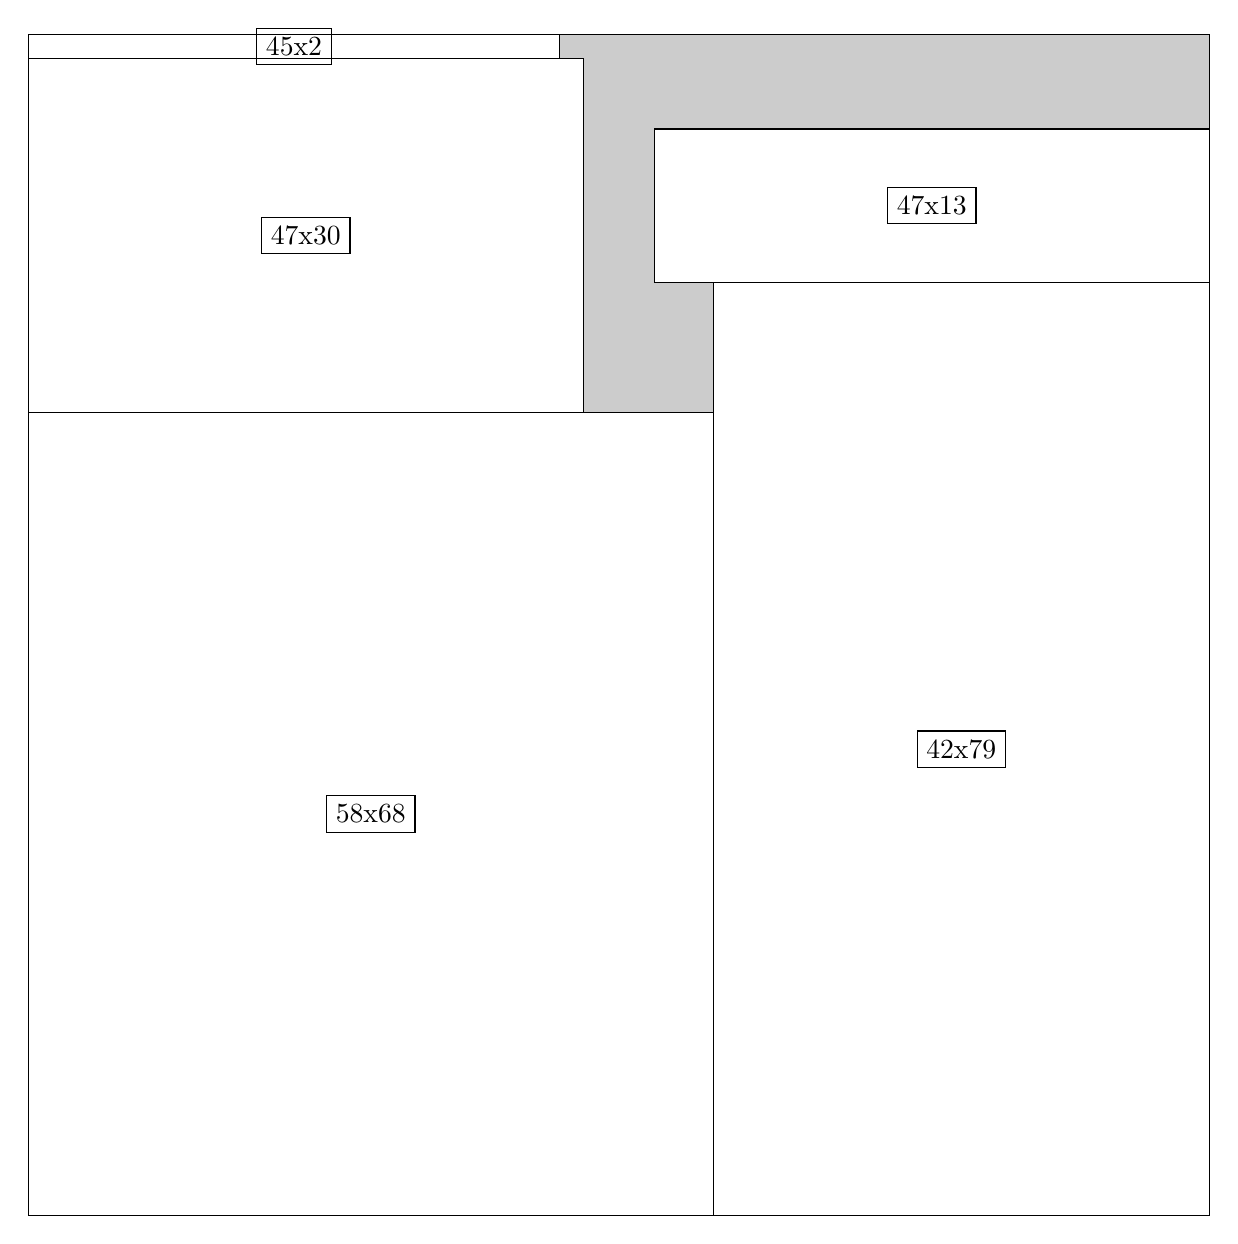
\begin{tikzpicture}[shorten >=1pt,scale=1.0,every node/.style={scale=1.0},->]
\tikzstyle{vertex}=[circle,fill=black!25,minimum size=14pt,inner sep=0pt]
\filldraw[fill=gray!40!white, draw=black] (0,0) rectangle (15.0,15.0);
\foreach \name/\x/\y/\w/\h in {58x68/0.0/0.0/8.7/10.2,42x79/8.7/0.0/6.3/11.85,47x30/0.0/10.2/7.05/4.5,47x13/7.949999999999999/11.85/7.05/1.95,45x2/0.0/14.7/6.75/0.3}
\filldraw[fill=white!40!white, draw=black] (\x,\y) rectangle node[draw] (\name) {\name} ++(\w,\h);
\end{tikzpicture}


w =58 , h =68 , x =0 , y =0 , v =3944
\par
w =42 , h =79 , x =58 , y =0 , v =3318
\par
w =47 , h =30 , x =0 , y =68 , v =1410
\par
w =47 , h =13 , x =53 , y =79 , v =611
\par
w =45 , h =2 , x =0 , y =98 , v =90
\par
\newpage


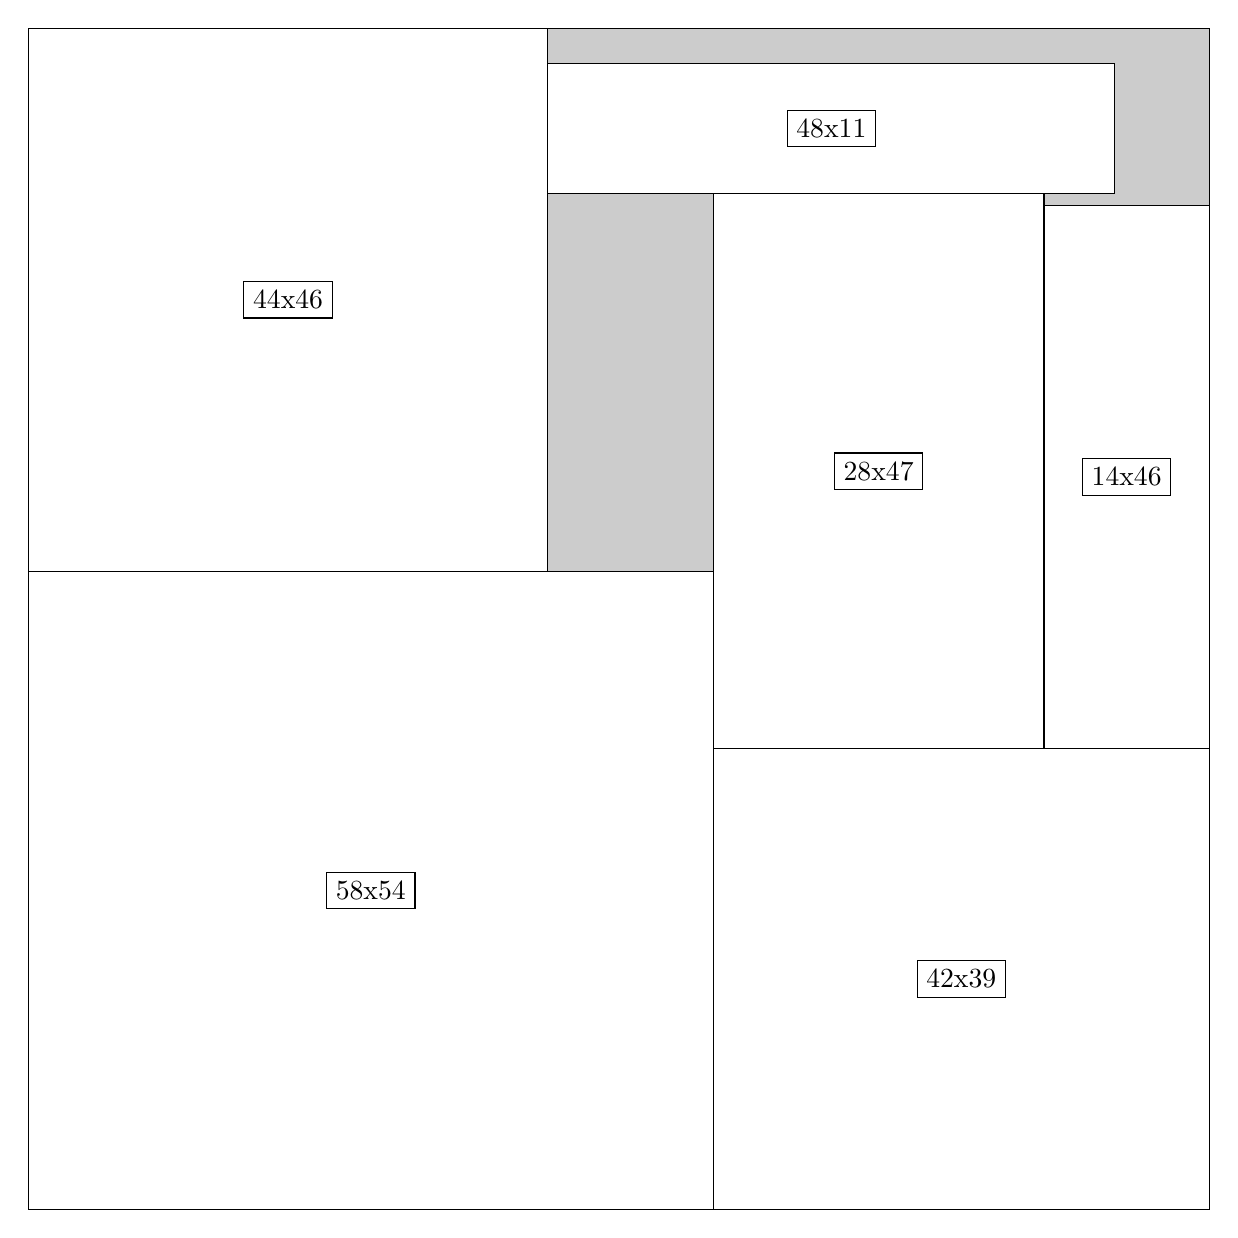
\begin{tikzpicture}[shorten >=1pt,scale=1.0,every node/.style={scale=1.0},->]
\tikzstyle{vertex}=[circle,fill=black!25,minimum size=14pt,inner sep=0pt]
\filldraw[fill=gray!40!white, draw=black] (0,0) rectangle (15.0,15.0);
\foreach \name/\x/\y/\w/\h in {58x54/0.0/0.0/8.7/8.1,44x46/0.0/8.1/6.6/6.8999999999999995,42x39/8.7/0.0/6.3/5.85,28x47/8.7/5.85/4.2/7.05,14x46/12.9/5.85/2.1/6.8999999999999995,48x11/6.6/12.9/7.199999999999999/1.65}
\filldraw[fill=white!40!white, draw=black] (\x,\y) rectangle node[draw] (\name) {\name} ++(\w,\h);
\end{tikzpicture}


w =58 , h =54 , x =0 , y =0 , v =3132
\par
w =44 , h =46 , x =0 , y =54 , v =2024
\par
w =42 , h =39 , x =58 , y =0 , v =1638
\par
w =28 , h =47 , x =58 , y =39 , v =1316
\par
w =14 , h =46 , x =86 , y =39 , v =644
\par
w =48 , h =11 , x =44 , y =86 , v =528
\par
\newpage


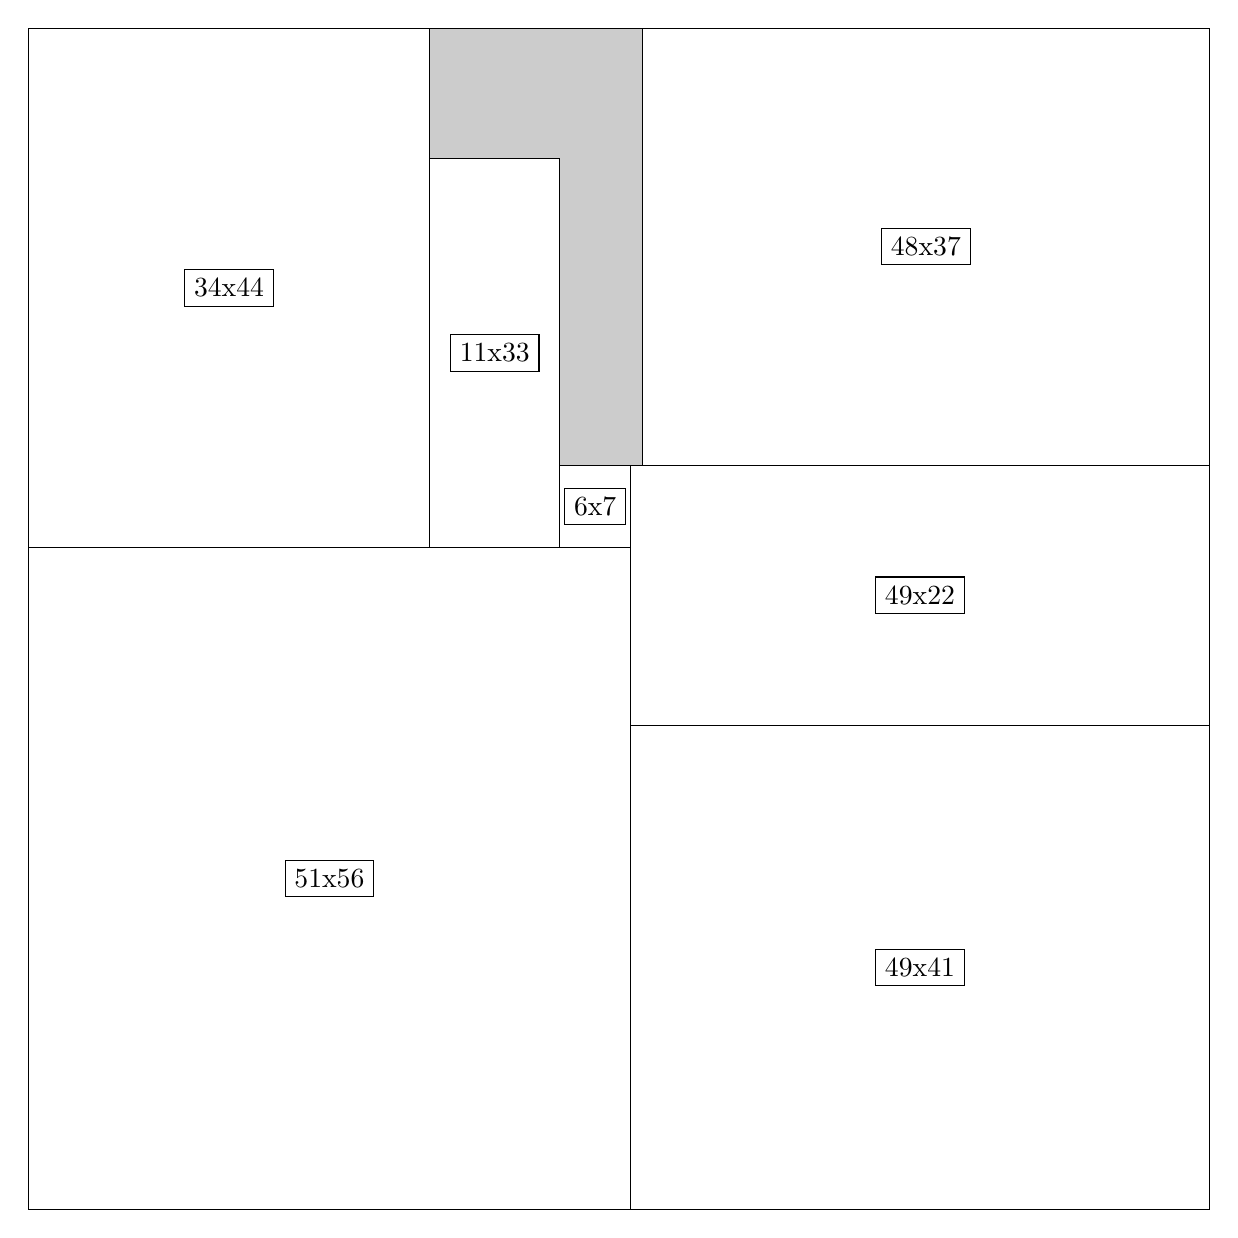
\begin{tikzpicture}[shorten >=1pt,scale=1.0,every node/.style={scale=1.0},->]
\tikzstyle{vertex}=[circle,fill=black!25,minimum size=14pt,inner sep=0pt]
\filldraw[fill=gray!40!white, draw=black] (0,0) rectangle (15.0,15.0);
\foreach \name/\x/\y/\w/\h in {51x56/0.0/0.0/7.6499999999999995/8.4,49x41/7.6499999999999995/0.0/7.35/6.1499999999999995,48x37/7.8/9.45/7.199999999999999/5.55,34x44/0.0/8.4/5.1/6.6,49x22/7.6499999999999995/6.1499999999999995/7.35/3.3,11x33/5.1/8.4/1.65/4.95,6x7/6.75/8.4/0.8999999999999999/1.05}
\filldraw[fill=white!40!white, draw=black] (\x,\y) rectangle node[draw] (\name) {\name} ++(\w,\h);
\end{tikzpicture}


w =51 , h =56 , x =0 , y =0 , v =2856
\par
w =49 , h =41 , x =51 , y =0 , v =2009
\par
w =48 , h =37 , x =52 , y =63 , v =1776
\par
w =34 , h =44 , x =0 , y =56 , v =1496
\par
w =49 , h =22 , x =51 , y =41 , v =1078
\par
w =11 , h =33 , x =34 , y =56 , v =363
\par
w =6 , h =7 , x =45 , y =56 , v =42
\par
\newpage


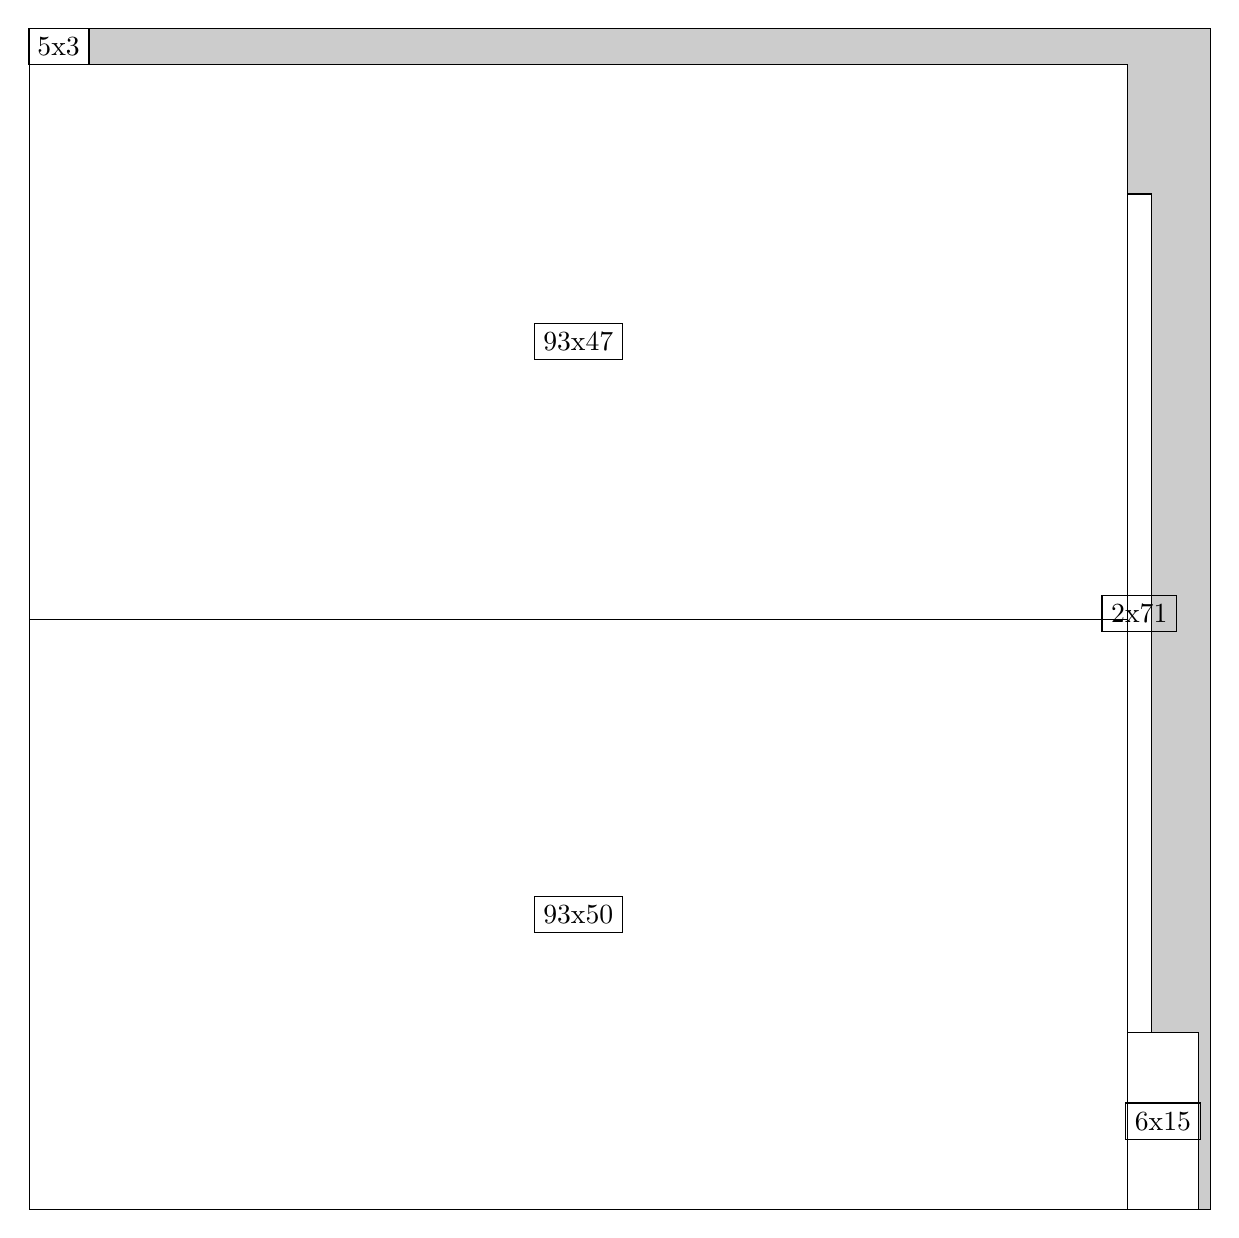
\begin{tikzpicture}[shorten >=1pt,scale=1.0,every node/.style={scale=1.0},->]
\tikzstyle{vertex}=[circle,fill=black!25,minimum size=14pt,inner sep=0pt]
\filldraw[fill=gray!40!white, draw=black] (0,0) rectangle (15.0,15.0);
\foreach \name/\x/\y/\w/\h in {93x50/0.0/0.0/13.95/7.5,93x47/0.0/7.5/13.95/7.05,2x71/13.95/2.25/0.3/10.65,6x15/13.95/0.0/0.8999999999999999/2.25,5x3/0.0/14.549999999999999/0.75/0.44999999999999996}
\filldraw[fill=white!40!white, draw=black] (\x,\y) rectangle node[draw] (\name) {\name} ++(\w,\h);
\end{tikzpicture}


w =93 , h =50 , x =0 , y =0 , v =4650
\par
w =93 , h =47 , x =0 , y =50 , v =4371
\par
w =2 , h =71 , x =93 , y =15 , v =142
\par
w =6 , h =15 , x =93 , y =0 , v =90
\par
w =5 , h =3 , x =0 , y =97 , v =15
\par
\newpage


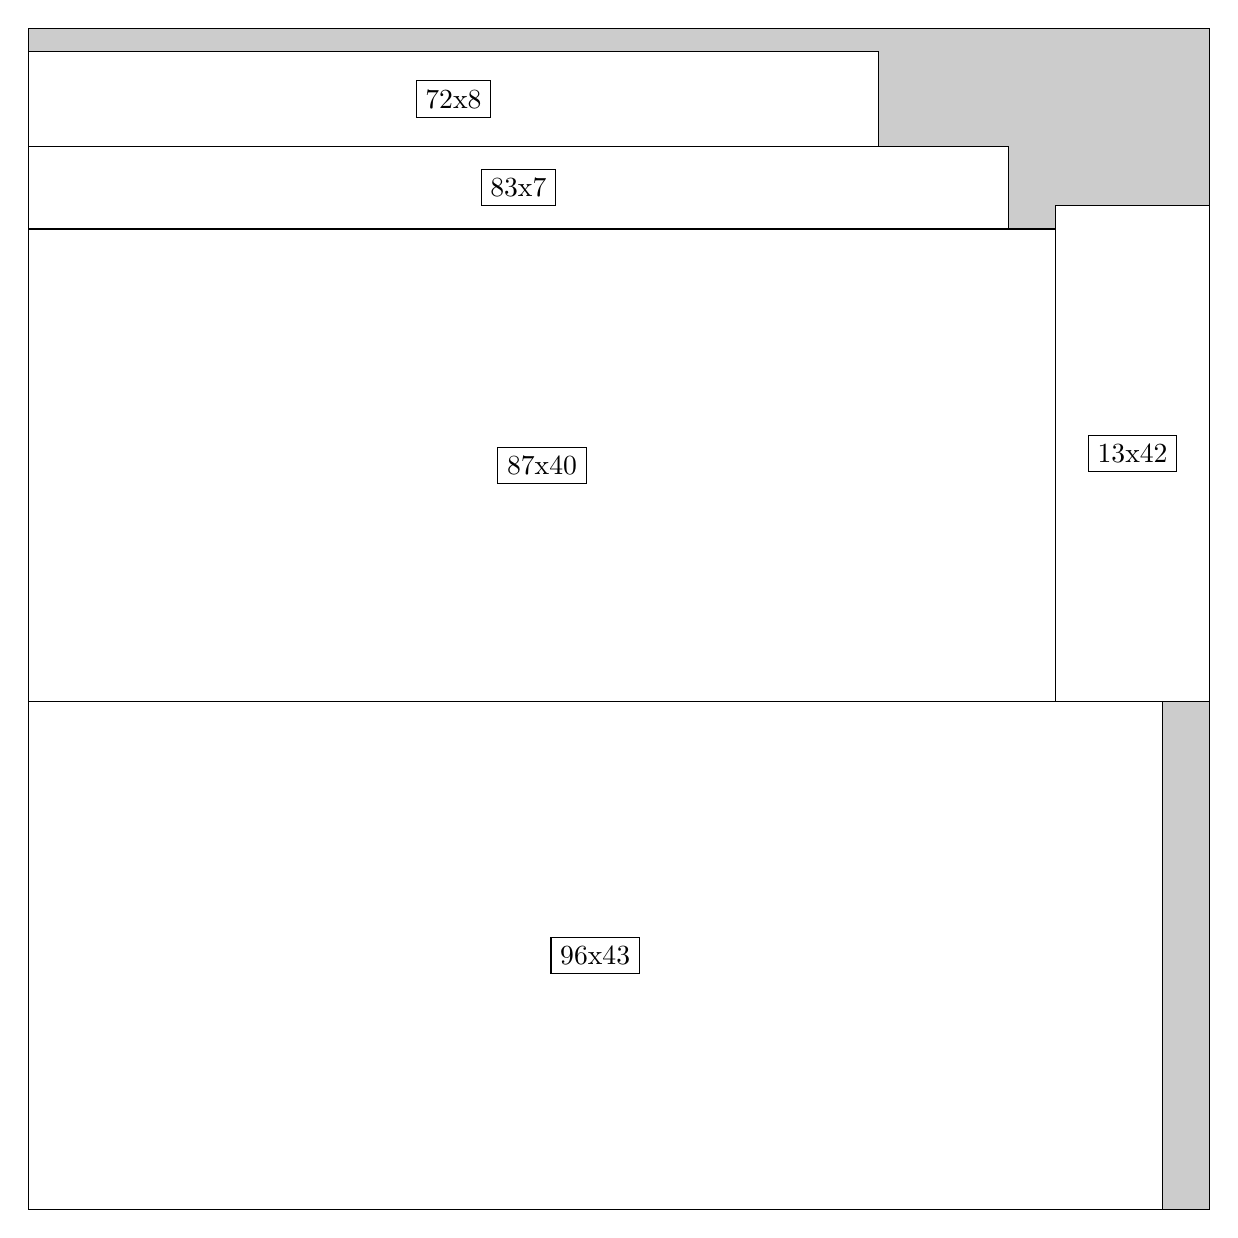
\begin{tikzpicture}[shorten >=1pt,scale=1.0,every node/.style={scale=1.0},->]
\tikzstyle{vertex}=[circle,fill=black!25,minimum size=14pt,inner sep=0pt]
\filldraw[fill=gray!40!white, draw=black] (0,0) rectangle (15.0,15.0);
\foreach \name/\x/\y/\w/\h in {96x43/0.0/0.0/14.399999999999999/6.45,87x40/0.0/6.45/13.049999999999999/6.0,83x7/0.0/12.45/12.45/1.05,72x8/0.0/13.5/10.799999999999999/1.2,13x42/13.049999999999999/6.45/1.95/6.3}
\filldraw[fill=white!40!white, draw=black] (\x,\y) rectangle node[draw] (\name) {\name} ++(\w,\h);
\end{tikzpicture}


w =96 , h =43 , x =0 , y =0 , v =4128
\par
w =87 , h =40 , x =0 , y =43 , v =3480
\par
w =83 , h =7 , x =0 , y =83 , v =581
\par
w =72 , h =8 , x =0 , y =90 , v =576
\par
w =13 , h =42 , x =87 , y =43 , v =546
\par
\newpage


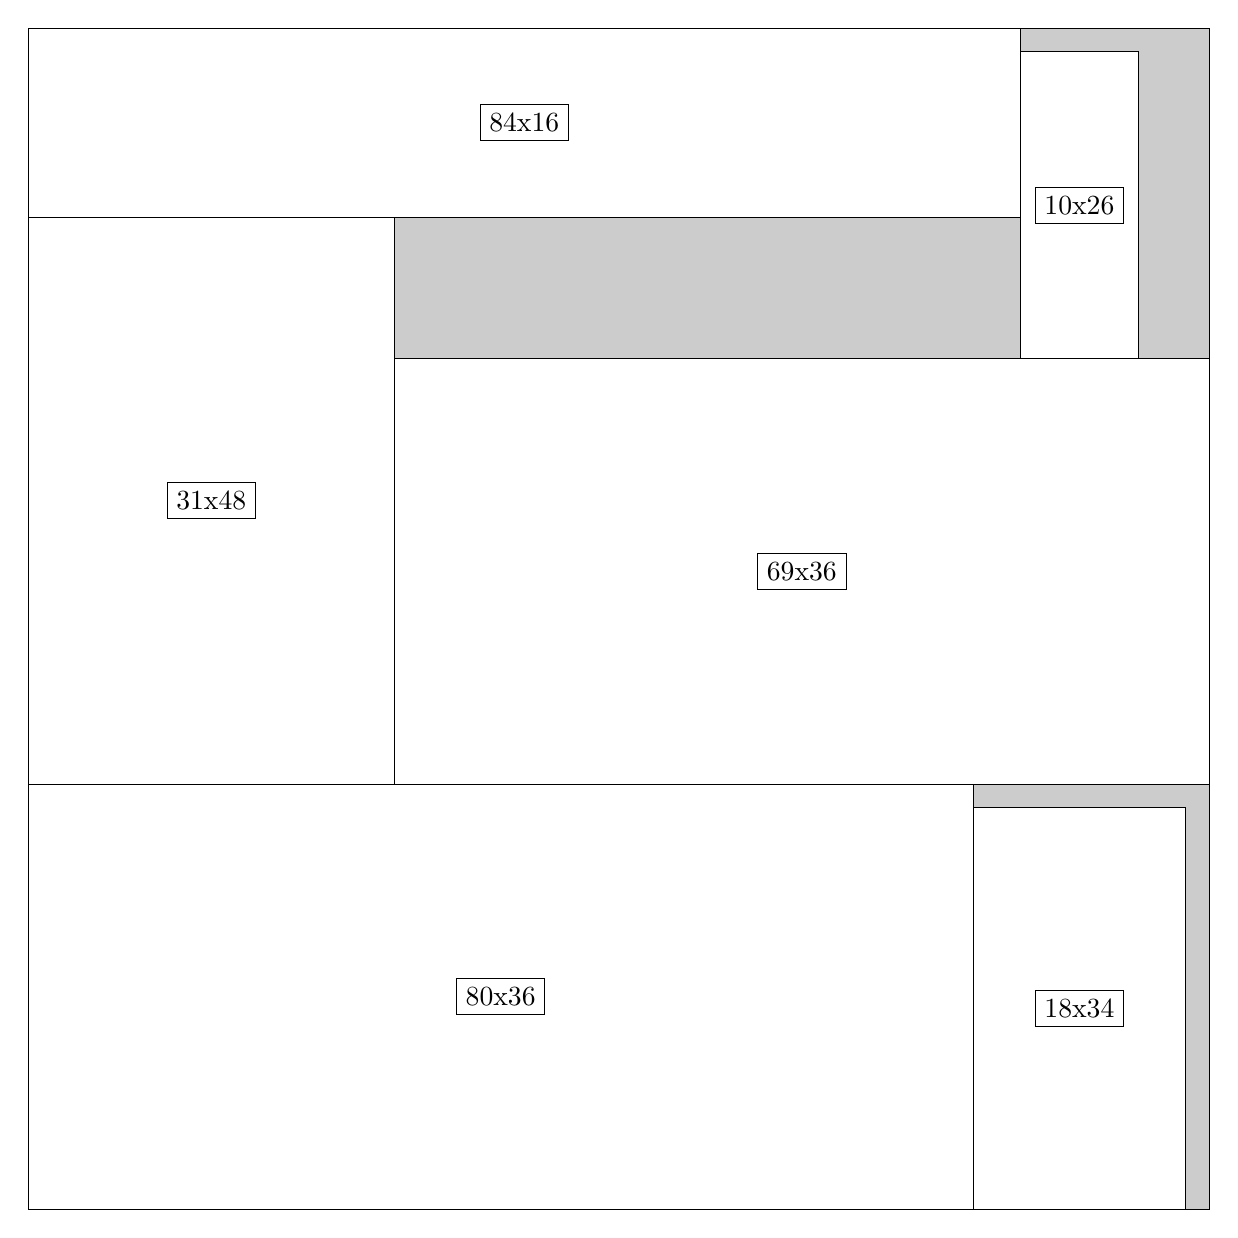
\begin{tikzpicture}[shorten >=1pt,scale=1.0,every node/.style={scale=1.0},->]
\tikzstyle{vertex}=[circle,fill=black!25,minimum size=14pt,inner sep=0pt]
\filldraw[fill=gray!40!white, draw=black] (0,0) rectangle (15.0,15.0);
\foreach \name/\x/\y/\w/\h in {80x36/0.0/0.0/12.0/5.3999999999999995,31x48/0.0/5.3999999999999995/4.6499999999999995/7.199999999999999,84x16/0.0/12.6/12.6/2.4,18x34/12.0/0.0/2.6999999999999997/5.1,10x26/12.6/10.799999999999999/1.5/3.9,69x36/4.6499999999999995/5.3999999999999995/10.35/5.3999999999999995}
\filldraw[fill=white!40!white, draw=black] (\x,\y) rectangle node[draw] (\name) {\name} ++(\w,\h);
\end{tikzpicture}


w =80 , h =36 , x =0 , y =0 , v =2880
\par
w =31 , h =48 , x =0 , y =36 , v =1488
\par
w =84 , h =16 , x =0 , y =84 , v =1344
\par
w =18 , h =34 , x =80 , y =0 , v =612
\par
w =10 , h =26 , x =84 , y =72 , v =260
\par
w =69 , h =36 , x =31 , y =36 , v =2484
\par
\newpage


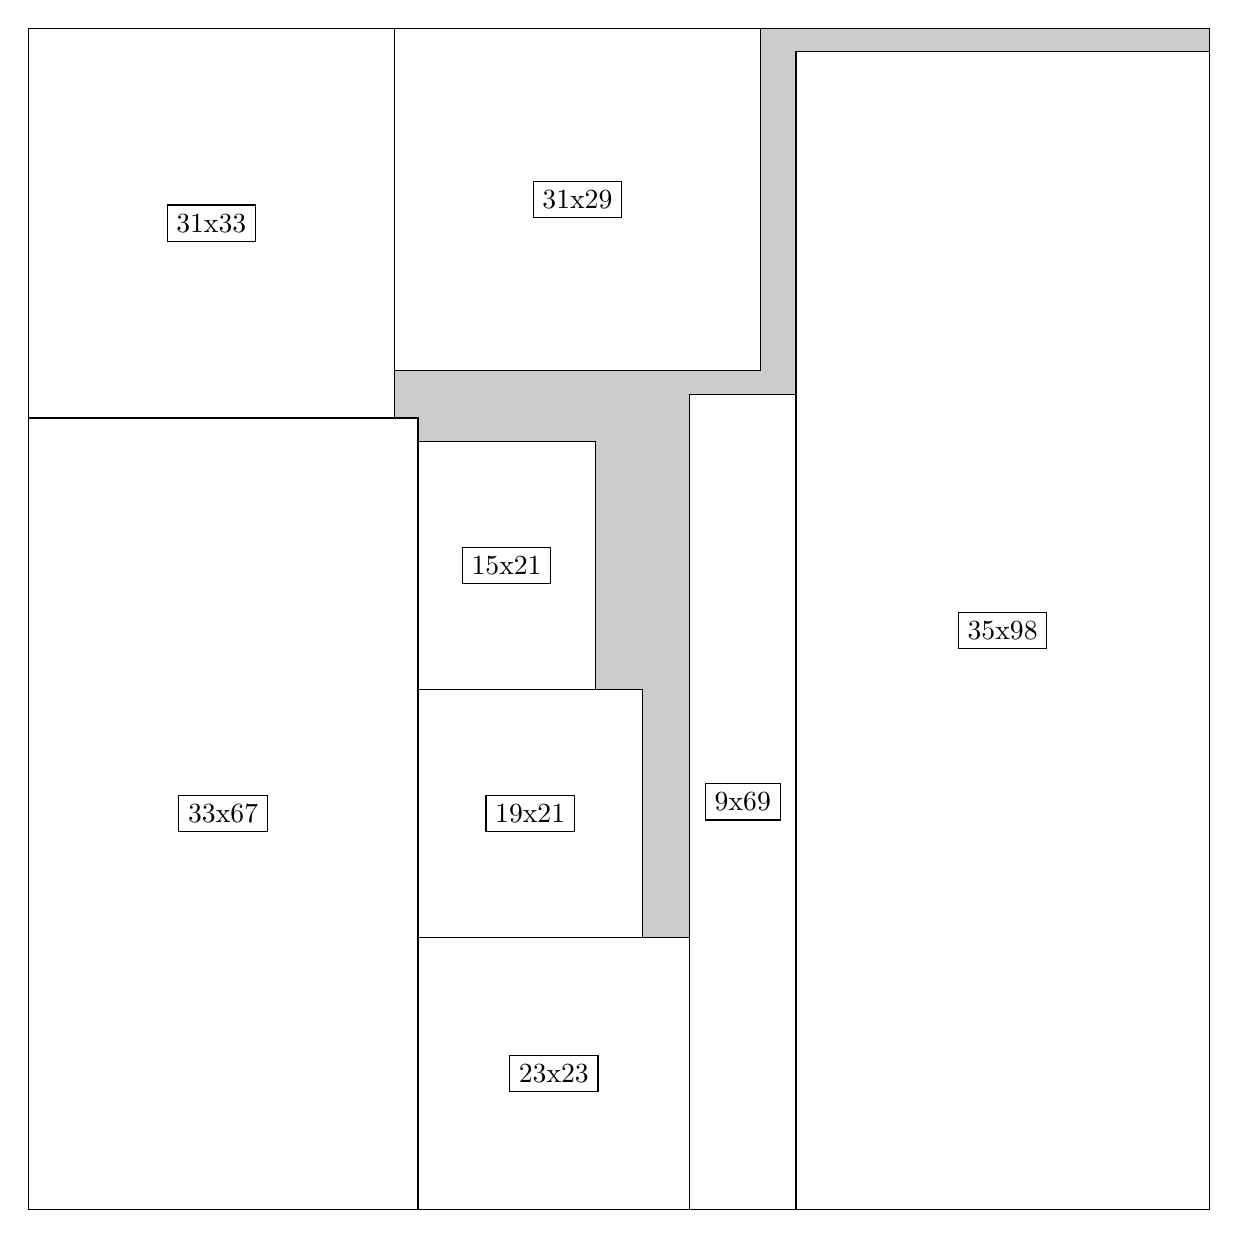
\begin{tikzpicture}[shorten >=1pt,scale=1.0,every node/.style={scale=1.0},->]
\tikzstyle{vertex}=[circle,fill=black!25,minimum size=14pt,inner sep=0pt]
\filldraw[fill=gray!40!white, draw=black] (0,0) rectangle (15.0,15.0);
\foreach \name/\x/\y/\w/\h in {35x98/9.75/0.0/5.25/14.7,33x67/0.0/0.0/4.95/10.049999999999999,23x23/4.95/0.0/3.4499999999999997/3.4499999999999997,31x29/4.6499999999999995/10.65/4.6499999999999995/4.35,9x69/8.4/0.0/1.3499999999999999/10.35,31x33/0.0/10.049999999999999/4.6499999999999995/4.95,19x21/4.95/3.4499999999999997/2.85/3.15,15x21/4.95/6.6/2.25/3.15}
\filldraw[fill=white!40!white, draw=black] (\x,\y) rectangle node[draw] (\name) {\name} ++(\w,\h);
\end{tikzpicture}


w =35 , h =98 , x =65 , y =0 , v =3430
\par
w =33 , h =67 , x =0 , y =0 , v =2211
\par
w =23 , h =23 , x =33 , y =0 , v =529
\par
w =31 , h =29 , x =31 , y =71 , v =899
\par
w =9 , h =69 , x =56 , y =0 , v =621
\par
w =31 , h =33 , x =0 , y =67 , v =1023
\par
w =19 , h =21 , x =33 , y =23 , v =399
\par
w =15 , h =21 , x =33 , y =44 , v =315
\par
\newpage


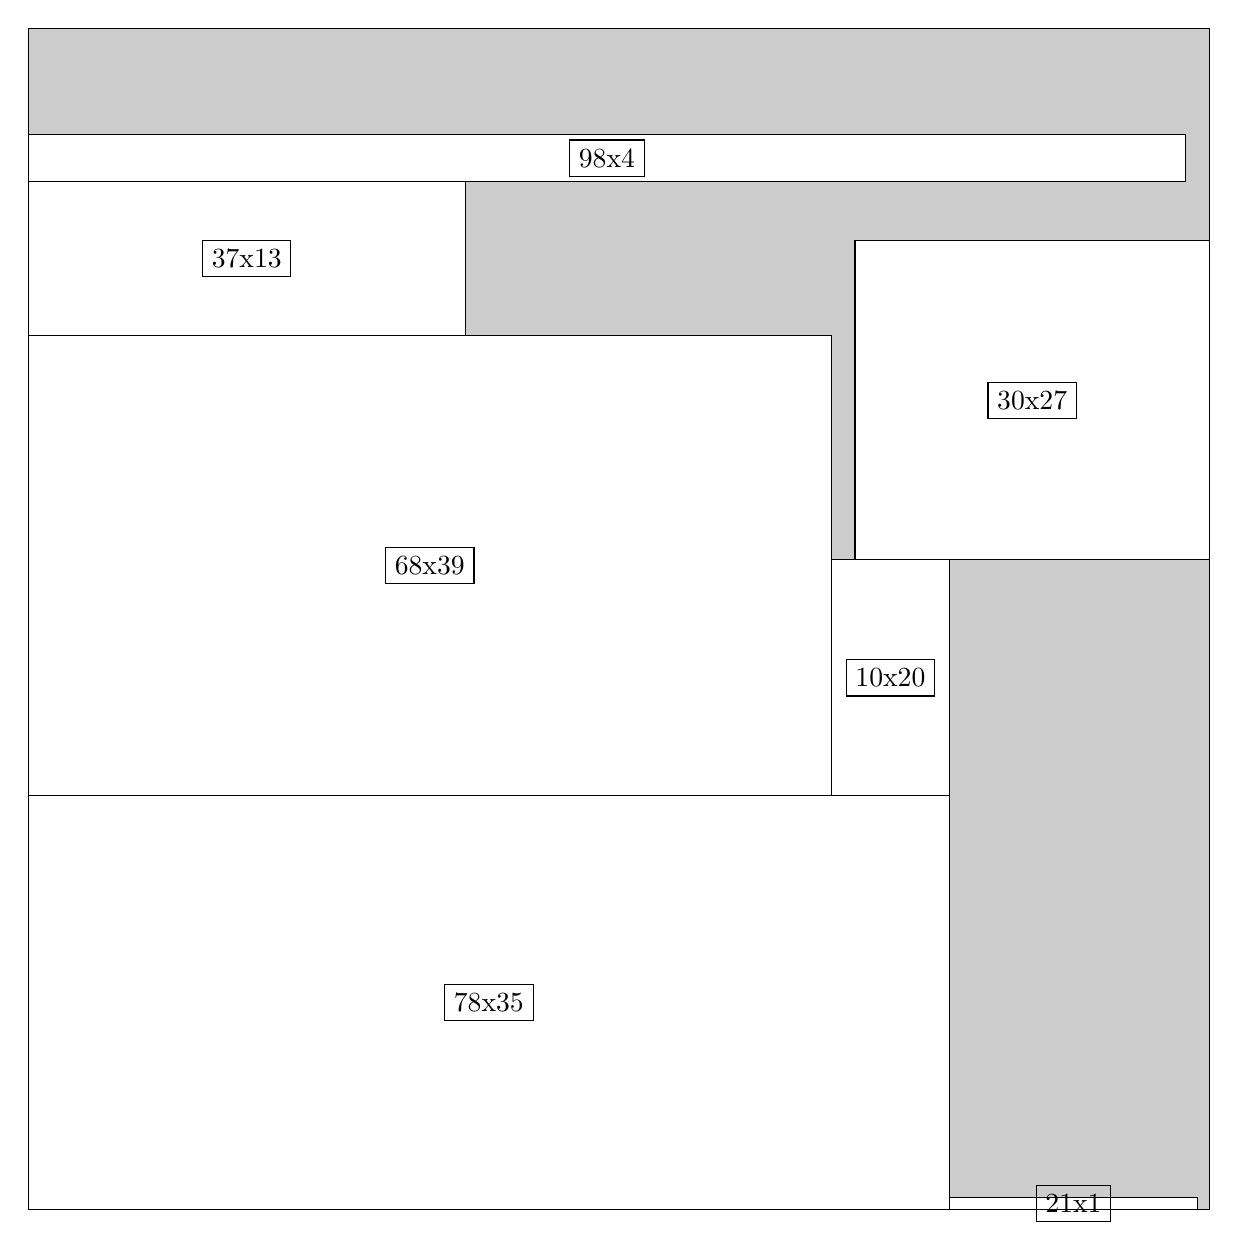
\begin{tikzpicture}[shorten >=1pt,scale=1.0,every node/.style={scale=1.0},->]
\tikzstyle{vertex}=[circle,fill=black!25,minimum size=14pt,inner sep=0pt]
\filldraw[fill=gray!40!white, draw=black] (0,0) rectangle (15.0,15.0);
\foreach \name/\x/\y/\w/\h in {78x35/0.0/0.0/11.7/5.25,68x39/0.0/5.25/10.2/5.85,30x27/10.5/8.25/4.5/4.05,37x13/0.0/11.1/5.55/1.95,98x4/0.0/13.049999999999999/14.7/0.6,10x20/10.2/5.25/1.5/3.0,21x1/11.7/0.0/3.15/0.15}
\filldraw[fill=white!40!white, draw=black] (\x,\y) rectangle node[draw] (\name) {\name} ++(\w,\h);
\end{tikzpicture}


w =78 , h =35 , x =0 , y =0 , v =2730
\par
w =68 , h =39 , x =0 , y =35 , v =2652
\par
w =30 , h =27 , x =70 , y =55 , v =810
\par
w =37 , h =13 , x =0 , y =74 , v =481
\par
w =98 , h =4 , x =0 , y =87 , v =392
\par
w =10 , h =20 , x =68 , y =35 , v =200
\par
w =21 , h =1 , x =78 , y =0 , v =21
\par
\newpage


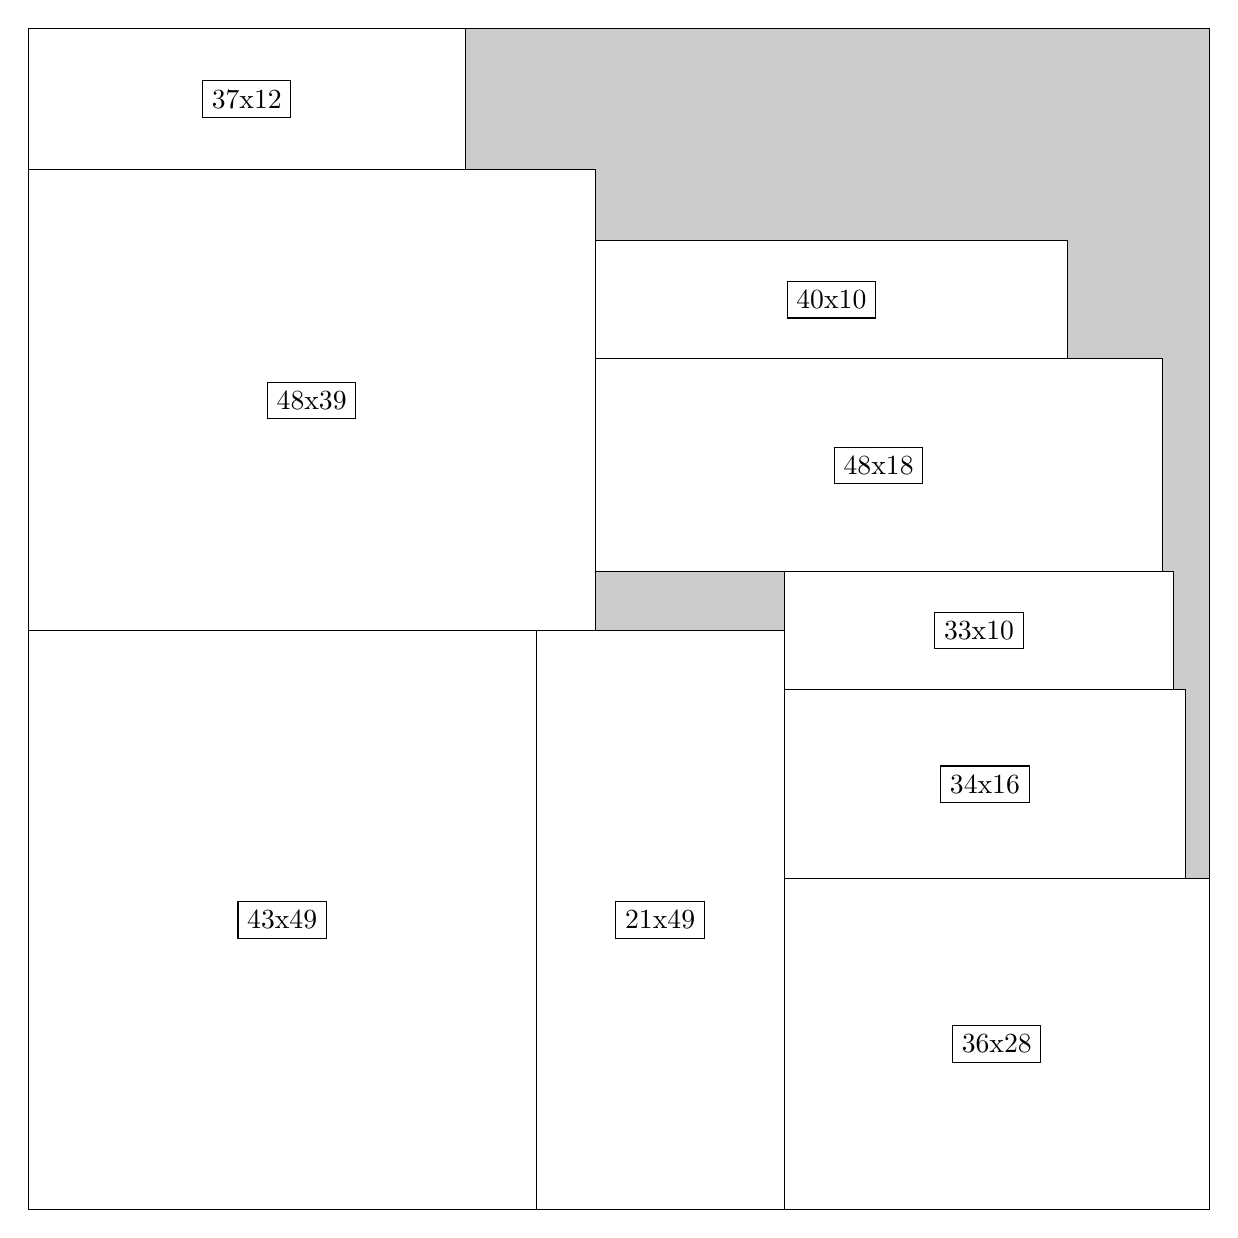
\begin{tikzpicture}[shorten >=1pt,scale=1.0,every node/.style={scale=1.0},->]
\tikzstyle{vertex}=[circle,fill=black!25,minimum size=14pt,inner sep=0pt]
\filldraw[fill=gray!40!white, draw=black] (0,0) rectangle (15.0,15.0);
\foreach \name/\x/\y/\w/\h in {43x49/0.0/0.0/6.45/7.35,48x39/0.0/7.35/7.199999999999999/5.85,21x49/6.45/0.0/3.15/7.35,36x28/9.6/0.0/5.3999999999999995/4.2,48x18/7.199999999999999/8.1/7.199999999999999/2.6999999999999997,34x16/9.6/4.2/5.1/2.4,37x12/0.0/13.2/5.55/1.7999999999999998,40x10/7.199999999999999/10.799999999999999/6.0/1.5,33x10/9.6/6.6/4.95/1.5}
\filldraw[fill=white!40!white, draw=black] (\x,\y) rectangle node[draw] (\name) {\name} ++(\w,\h);
\end{tikzpicture}


w =43 , h =49 , x =0 , y =0 , v =2107
\par
w =48 , h =39 , x =0 , y =49 , v =1872
\par
w =21 , h =49 , x =43 , y =0 , v =1029
\par
w =36 , h =28 , x =64 , y =0 , v =1008
\par
w =48 , h =18 , x =48 , y =54 , v =864
\par
w =34 , h =16 , x =64 , y =28 , v =544
\par
w =37 , h =12 , x =0 , y =88 , v =444
\par
w =40 , h =10 , x =48 , y =72 , v =400
\par
w =33 , h =10 , x =64 , y =44 , v =330
\par
\newpage


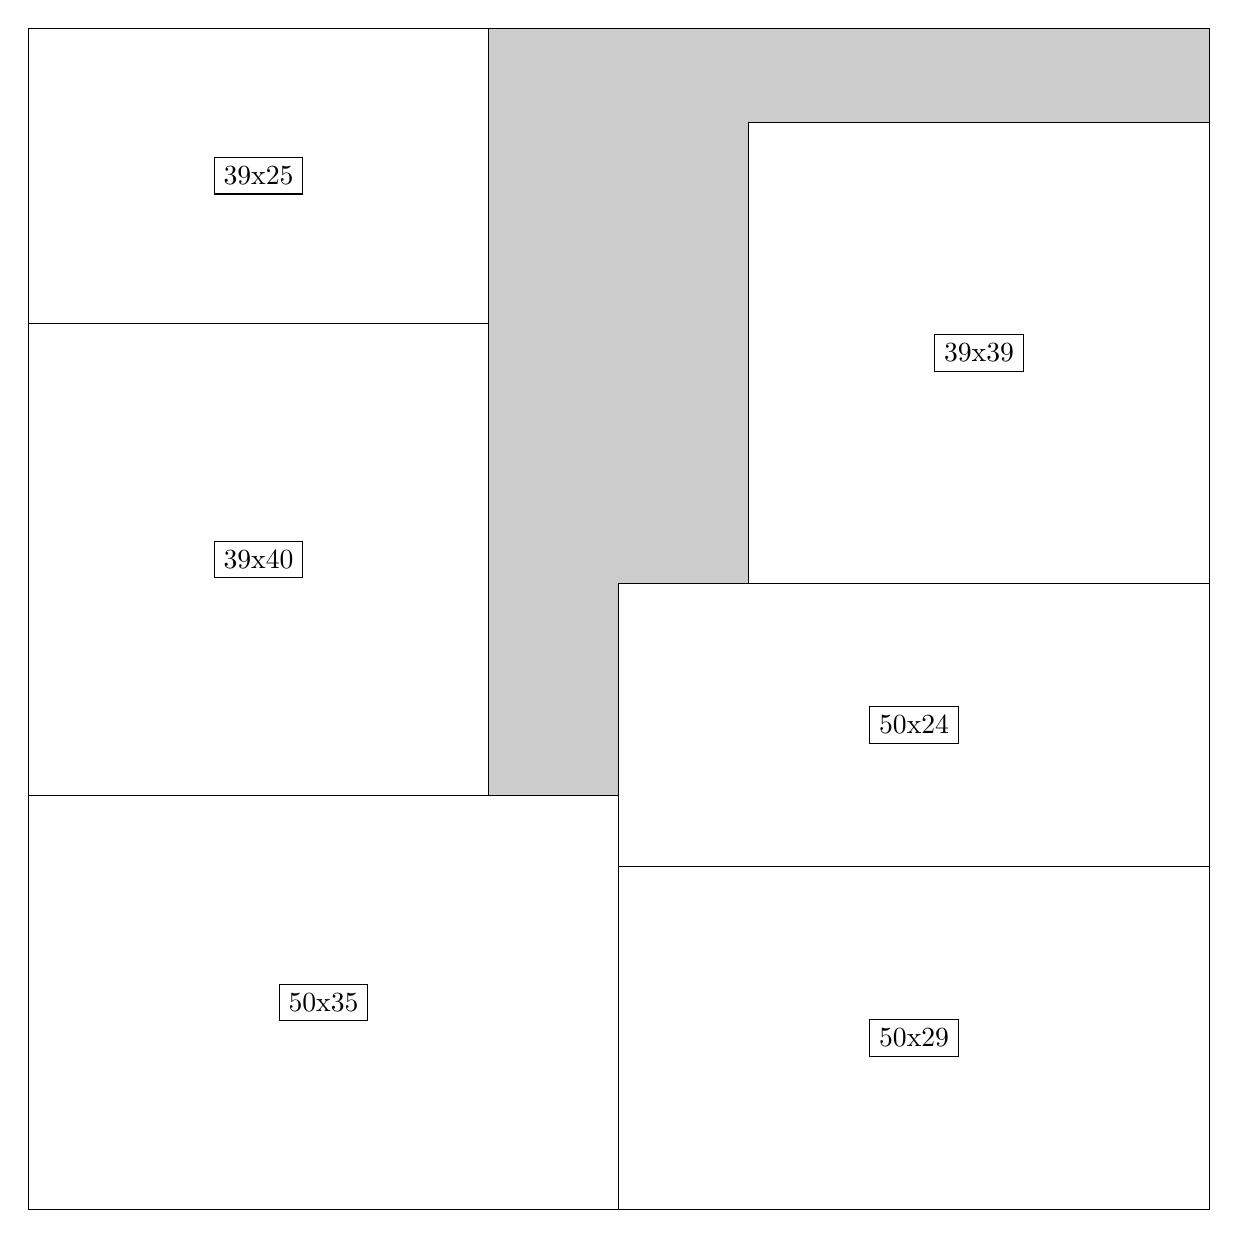
\begin{tikzpicture}[shorten >=1pt,scale=1.0,every node/.style={scale=1.0},->]
\tikzstyle{vertex}=[circle,fill=black!25,minimum size=14pt,inner sep=0pt]
\filldraw[fill=gray!40!white, draw=black] (0,0) rectangle (15.0,15.0);
\foreach \name/\x/\y/\w/\h in {50x35/0.0/0.0/7.5/5.25,39x40/0.0/5.25/5.85/6.0,39x39/9.15/7.949999999999999/5.85/5.85,50x29/7.5/0.0/7.5/4.35,50x24/7.5/4.35/7.5/3.5999999999999996,39x25/0.0/11.25/5.85/3.75}
\filldraw[fill=white!40!white, draw=black] (\x,\y) rectangle node[draw] (\name) {\name} ++(\w,\h);
\end{tikzpicture}


w =50 , h =35 , x =0 , y =0 , v =1750
\par
w =39 , h =40 , x =0 , y =35 , v =1560
\par
w =39 , h =39 , x =61 , y =53 , v =1521
\par
w =50 , h =29 , x =50 , y =0 , v =1450
\par
w =50 , h =24 , x =50 , y =29 , v =1200
\par
w =39 , h =25 , x =0 , y =75 , v =975
\par
\newpage


\end{document}